%flowchart%%%%%%%%%%%%%%%%%%%%%%%%%%%%%%%%%%%%%%%%%%%%%%%%%%%%%%%%%%%%%%%%%%%%%%%%%%%%%%%%
%2345678901234567890123456789012345678901234567890123456789012345678901234567890
%        1         2         3         4         5         6         7         8

\documentclass[letterpaper, 10 pt, conference]{ieeeconf}  % Comment this line out if you need a4paper

%\documentclass[a4paper, 10pt, conference]{ieeeconf}      % Use this line for a4 paper

\IEEEoverridecommandlockouts                              % This command is only needed if 
                                                          % you want to use the \thanks command

\overrideIEEEmargins                                      % Needed to meet printer requirements.

% See the \addtolength command later in the file to balance the column lengths
% on the last page of the document

% The following packages can be found on http:\\www.ctan.org
%\usepackage{graphics} % for pdf, bitmapped graphics files
%\usepackage{epsfig} % for postscript graphics files
%\usepackage{mathptmx} % assumes new font selection scheme installed
%\usepackage{times} % assumes new font selection scheme installed
\usepackage{amsmath} % assumes amsmath package installed
%\usepackage{amssymb}  % assumes amsmath package installed
\usepackage{graphicx}
\usepackage{times,ifthen}
\usepackage{algorithm}
\usepackage{algorithmic}
%\usepackage{algorithmicx}

\title{\LARGE \bf
 Distributed network localization
}


\author{Laurent Fasnacht Matteo Pagliardini Bernard Maccari% <-this % stops a space
%\thanks{*This work was not supported by any organization}% <-this % stops a space
%\thanks{$^{1}$Albert Author is with Faculty of Electrical Engineering, Mathematics and Computer Science,
%        University of Twente, 7500 AE Enschede, The Netherlands
%        {\tt\small albert.author@papercept.net}}%
%\thanks{$^{2}$Bernard D. Researcheris with the Department of Electrical Engineering, Wright State University,
 %       Dayton, OH 45435, USA
%        {\tt\small b.d.researcher@ieee.org}}%
}


\begin{document}



\maketitle
\thispagestyle{empty}
\pagestyle{empty}


%%%%%%%%%%%%%%%%%%%%%%%%%%%%%%%%%%%%%%%%%%%%%%%%%%%%%%%%%%%%%%%%%%%%%%%%%%%%%%%%
\begin{abstract}
This paper presents an implementation of a distributed algorithm for localizing static sensor nodes in a two-dimensional network. Nodes can sense noisy distances to neighboring nodes and communicate asynchronously with them. Our method follow the work of David Moore $et$ $al.$ \cite{MooreTeller}. We evaluate our method in term of speed of convergence and precision of the estimated positions. \\
Using simulation we show that this method approximates well the position in a fairly noisy environment. We also show the robustness of the method against perturbations such as nodes displacements. The algorithm is able to cleverly select anchor points and thus is adequat for applications where the user has no control over nodes' position. Finally the algorithm is fully distributed.
moo\end{abstract}


%%%%%%%%%%%%%%%%%%%%%%%%%%%%%%%%%%%%%%%%%%%%%%%%%%%%%%%%%%%%%%%%%%%%%%%%%%%%%%%%
\section{INTRODUCTION}

Self-localization is a fundamental need in networks. With numerous military and civilian applications such as environmental monitoring or surveillance.  Distributed algorithms offer a way to divide the computational burden and to minimize the overall cost of communication. It also greatly enhances the robustness of the overall system. 

We present a solution to localize a network of static sensor nodes. The nodes can sense noisy distances to neighboring nodes and are also capable of communicating with their neighbors. We consider the quality of the algorithm looking at several criteria such as precision, speed of convergence, stability, resistance to perturbations, scalability and computational cost. A good localization algorithm has to balance all of these aspects.

The localization problem is non-trivial since each node pocesses only a very limited knowledge of the system and the solution pool for a node might be large. This is emphasized when the noise over measurement increases. Another difficulty comes from the lack of control over the nodes' position which generate additional difficulties concerning the choice of initials anchor points. Finally the entire system being distributed we have very limited communications abilities. 

We use the idea of David Moore $et$ $al.$ \cite{MooreTeller} to rely on properties of quadrilaterals to solve flip ambiguities. Flex ambiguities are solved defining the notion of robust quadrilaterals. A quadrilateral is robust when all vertices are connected to all others and when for all triangles $b*sin(min_i \theta_i)^2 > d_{min} $ where $\theta_i$ are the angles and $b$ the smallest side. We diverge from \cite{MooreTeller} on several details but most notably on the cluster definition and transformation parts. these modifications makes our algorithm fully distributed i.e. every node does the same set of operations.

Our method demonstrated the following capabilities : INSERT RESULTS HERE | INSERT RESULTS HERE | INSERT RESULTS HERE | INSERT RESULTS HERE | INSERT RESULTS HERE | INSERT RESULTS HERE | INSERT RESULTS HERE | INSERT RESULTS HERE | INSERT RESULTS HERE | INSERT RESULTS  

\section{Experiments}

During the developement of the project we sometime diverged from Moore $et$ $al.$ 's implementation. We've also made very specific implementation choices that we will discuss in this section. Finally we verified our choices using simple regular graphs.

\subsection{Modifications over Moore $et$ $al.$ 's implementation}

%%%%%%%%%%%%%%%%%%%%%%%%%%%% ROBUST QUADS %%%%%%%%%%%%%%%%%%%%%%%%%%%%%%%%%%%%%%%%%%%%%%%%
The first step was to detect all robust-quads for a given node. In \cite{} the algorithm used to iterates over all the nodes with a depth of 4 from the current node. The 4 nested loops yield an $O(n^4)$ complexity. It is in fact possible only to consider a depth of 3 knowing that the last edge need to link to the current node. This in mind we've implemented an algorithm to find all robust-quads containing a node with a cubic complexity. Saving computational time is part of the important aspect of a good solution. The implemented algorithm is presented as Algorithm 1. 

\begin{algorithm}[H]
\caption{Find robust quads of node $i$. This algorithm loops over each triplet of neighbours of the node $i$ and find if the resulting quad is robust. $quadIsRobust$ checks if the quad is fully connected, and if each triangle of the quad is robust.}
\begin{algorithmic} 
\STATE $neighboursIds \leftarrow neighbors(node(i))$
\STATE $nbneighbours \leftarrow length(neighboursIds)$ 
\STATE $robustQuadsList \leftarrow []$ 
\FOR  {$j_i=0$ to $ nbneighbours $} 
\FOR  {$k_i=j_i+1$ to $ nbneighbours $} 
\FOR  {$l_i=k_i+1$ to $ nbneighbours $} 
\STATE $j \leftarrow neighboursIds(j_i)$ 
\STATE $k \leftarrow neighboursIds(k_i)$
\STATE $l \leftarrow neighboursIds(l_i)$ \newline
\IF {$quadIsRobust(i,j,k,l)$} 
\STATE $robustQuadsList \leftarrow [i, j, k, l]$
\ENDIF 
\newline
\ENDFOR
\ENDFOR
\ENDFOR 
\STATE $node(i).robustquads \leftarrow robustQuadsList$
\end{algorithmic}
\end{algorithm}

%%%%%%%%%%%%%%%%%%%%%%%%%%%% VAR ESTIMATION %%%%%%%%%%%%%%%%%%%%%%%%%%%%%%%%%%%%%%%%%%%%%%%
In \cite{} the variance of the noise is used to compute $d_{min}$. Its value is fixed and identical for every node. This implied that the noise is known in advanced and that each node has to be calibrated with this value. Based on \cite{Knuth} we've implemented a method allowing each node to estimate the variance they see over the measurements. This emphasize the fully distributed approach we choose to adopt for this project.\newline

%%%%%%%%%%%%%%%%%%%%%%%%%%%% SIGMA EDGE LENGTH %%%%%%%%%%%%%%%%%%%%%%%%%%%%%%%%%%%%%%%%%%%%%
Note that our definition of robust differs from \cite{}. In our implementation, the variance on the noise is proportional to the length of the edge. As $d_{min}$ is choosen with respect to the noise, we already consider the length the shortest edge when we compute $d_{min}$. \newline

%%%%%%%%%%%%%%%%%%%%%%%%%%%% SPRING RELAXATION %%%%%%%%%%%%%%%%%%%%%%%%%%%%%%%%%%%%%%%%%%%%%
As proposed in \cite{}, we have inplemented the spring relaxation technique to see how it can improve performances. Spring relaxation computes the forces applied to each nodes by its neighbours. Each force is proportional to the difference between the distances measured and the distances computed with the positions of the nodes. Then we compute the position that minimize the potential.
The node uses both robust squad and spring relaxation techniques with appropriate weigths to compute its new position. The performances of this optimization is discussed in the result section. 
\newline

%%%%%%%%%%%%%%%%%%%%%%%%%%%% ANCHOR NODE ESTI. %%%%%%%%%%%%%%%%%%%%%%%%%%%%%%%%%%%%%%%%%%%%%
In \cite{} the positions are propagated by associating a cluster to each node and solving the best rotation and translation to merge these clusters. This implies a lot of information sharing among the nodes and represents to us a flaw in the distributed scheme we wanted. We've decided to modify this part of the implementation for a fully distributed version relying on anchor nodes to propagate the position starting from an origin. The user might not be able to modify the nodes' position and we must be careful not to select bads anchor nodes i.e. starting nodes from which we cannot propagate. To realise this we dynamically select the anchor points by propagating a score in the network. For each node this score represents how regular and numerous the robust-quads are at this node. The anchor points are selected from the best scoring node. 

The propagation step then works as follow : for each node we consider computing its position looking at the set of robust quadrilaterals the point belongs to. The three anchor nodes fix an arbitrary translation, rotation, and reflection. The origin node is set as origin of the coordinate system. A node trilaterates its position when he belongs to a robust-quad containing three points of known position. When several robust-quads are available we select the best one. Here the notion of best is defined as the smallest distance from the node of the robust quad to the source. Indeed, the robust-quads closer to the origin are more reliable than the one far away. This priority is essential for the convergence of the algorithm, it ensures that the propagation will always occur starting from the source.

MORE DETAILS NEEDED HERE ABOUT SELECTING THE BEST QUAD AND WHAT HAPPEN WHEN ANCHORS CHANGE + DIAGRAM

As a consequence of this choice we only have one relative coordinate system for all of our nodes instead of one coordinate system for each node as in Moore $et$ $al.$'s implementation. 

\subsection{Implementation choices}

%%%%%%%%%%%%%%%%%%%%%%%%%%%% FULLY DISTRIBUTED %%%%%%%%%%%%%%%%%%%%%%%%%%%%%%%%%%%%%%%%%%%%%
To validate an entirely distributed model, each node has private data, only accesible through communication. For a node the knowledge of the network is sparse and limited to his neignbors. No global information sharing is done as in \cite{}. Thus our implementation is cheap in term of memory requirement. Each node has a probability of evaluating its distance to his neighbors, when a new measurement is done the new values are broadcast.\newline


%%%%%%%%%%%%%%%%%%%%%%%%%%%% COMPUTATION THEN COM %%%%%%%%%%%%%%%%%%%%%%%%%%%%%%%%%%%%%%%%%%
A network localization problem relies on local communications and tries to solve a global task. Thus the first step of our work was actually to model the exchanges happening between different nodes. We model this by a two states machine. The first step is communication, the nodes send different types of messages to neighbors:

\begin{itemize}

\item measured distances to its neighbours
\item its absolute position
\item its list of robust quads. %need to give more details about why ? 
% !!!! TO BE REPLACED?
\item its distance to the origin of the graph, defined in numbers of hops to it.

\end{itemize}

During the second stage the message are processed. These two alternated steps ensure a realistic simulation where the information is processed at each timer tick. 

INSERT DIAGRAM : enumerate all possible messages / agencer avec node\_timer\_tick

\subsection{Parameters introduced}

%%%%%%%%%%%%%%%%%%%%%%%%%%%% PARAMETERS LIST %%%%%%%%%%%%%%%%%%%%%%%%%%%%%%%%%%%%%%%%%%%%%%%
Our implementation choices made us introduce new parameters. 

\begin{itemize}
\item $d_{min}$ factor : ratio between the threshold dmin and the variance of the noise
\item spring relaxation factor : weigth in the interpolation between the m distance to the origin of the graph, defined in numbers of hops to it.
\end{itemize}


\subsection{Tests on regular graphs}

We tried to set up a simple regular network used to trivially verify our implementation emoving the uncertainty infered by the graph topology. These graph can as well be used as reference graphs used to compare with more complicated graphs.\newline


\begin{figure}[ht!]
\centering
%\includegraphics[width=90mm]{}
\caption{regular graph}
\end{figure}


\section{Results}
%speed of convergence
%Performance Metrics
%Scalability : performances w.r.t Nb of nodes

\section{Conclusion}










%%%%%%%%%%%%%%%%%%%%%%%%%%%%%%%%%%%%%%%%%%%%%%%%%%%%%%%%%%%%%%%%%%%%%%
%%%%%%%%%%%%%%% UNDER THIS LINE : OLD STUFF %%%%%%%%%%%%%%%%%%%%%%%%%%
%%%%%%%%%%%%%%%%%%%%%%%%%%%%%%%%%%%%%%%%%%%%%%%%%%%%%%%%%%%%%%%%%%%%%%
OLD STUFF
OLD STUFF
OLD STUFF
OLD STUFF
OLD STUFF














\subsection{Error measurement}
We measure the error on the distances 
%sigma_p
%sigma_d



%spring relaxation :smooth error + decrease convergence speed if bad initalization

\subsection{Perturbations}

\subsection{Shortcomings}
%

\section{Conclusion}


\begin{thebibliography}{99}

\bibitem{MooreTeller} Moore Teller, ÒSynthetic structure of industrial plastics (Book style with paper title and editor),Ó 	in Plastics, 2nd ed. vol. 3, J. Peters, Ed.  New York: McGraw-Hill, 1964, pp. 15Ð64.

\bibitem{Knuth} David Moore John Leonard Daniela Rus Seth Teller, ÒRobust Distributed Network Localization with Noisy Range Measurements, 2004.




\end{thebibliography}








In our implementation the graph can be completely random, however experiments showed that a connectivity threshold of XXX was required to ensure good performances. As in \cite{MooreTeller} we use properties of quadrilaterals to answer the flip ambiguity problem. The flex ambiguity is solved selecting only robust quadrilaterals having a "good" shape considering the noise level, this notion will be defined later on. 

The last step of the algorithm is to determine the position of the nodes from those robust quads. We diverge here from \cite{MooreTeller} by cleverly selecting anchor nodes and propagating the position using trilateration. A spring relaxation technique is used to refine the solution. 

   \begin{figure}[thpb]
      \centering
      \framebox{\parbox{3in}{ 
      Insert diagram that recap the main steps
      \\\\\\\\\\\\\\\\\\\\\\\\\\\\\\\\
}}
      %\includegraphics[scale=1.0]{figurefile}
      \caption{Main steps done by the algorithm, note once again that all is done in a distributed fashion}
      \label{figurelabel}
   \end{figure}


%detail each point and introduce briefly our approach.

%for each point say how we answer the problem 

%

\subsection{Communication}
% detail how the information is shared among the nodes / small talk about memory requirements / cost of com (energy)
Communication is a critial aspect in distributed systems. It is the most expensive and time consuming part. Each node can communicate only with its neighbors, they have a certain probability to do distances measurements. When a measurement has been realized they broadcast the new information to all their neighbors.

Our algorithm uses anchor nodes from which it propagates the positions. When these special nodes have been selected we need additional information to propagate correctly. Points' localization is achieved using trilateration when a point belong to a robust quadrilateral. Because one point can belong to several such quadrilaterals we use the distance to the source to define a priority among solutions. The information closer to the source being more reliable we use quadrilaterals with the smallest distance to the source to trilaterate the position. The distance to the origin has to be computed for each node, we diffuse this information from the origin of the network. Each node look at their neighbors and update their distance as 1 if one them is the source or $min_i(neighbor_i.distance) +1 $ in the other case. This takes few seconds for all the nodes to guess their distance.

ADD COMMENT ON SELECTING THE ANCHOR NODE

\subsection{Information of node}

Keeping in mind the criterion of energy minimization, each node store data about itself and its neighbours. With a certain probabily , and if they are available, the node share with its neighbours the following informations :

\begin{itemize}

\item measured distances to the neighbours
\item its absolute position
\item its list of robust quads.
\item its distance to the origin of the graph, defined in numbers of hops to it.

\end{itemize}

The later is useful to select the most reliable robusts-quad among the ones available to the node.

% average on measures of distances.

\subsection{Robust quad}
%why using it
A common problem in localization based on distances is flip ambiguities. A flip ambiguity create two possible localizations that both satisfy the distances constraints. Two prevent that, we use the concept presented in \cite{MooreTeller} of robust quads.
A robust quad is a quadrilateral where each vertex are connected with all others.
With non-noisy distances measurements, robust quads offer the possibility build a unique graph. However, in precense of noise, we must add a constraint on angles to reduce the probability of flip ambiguities.
Therefore to this definition, we add the constraint to reduce the probability of a flip ambiguity. This constraint states that every angle of the quad is larger than a threshold. 
Q robust quad can also be seen as a set of four robust triangles. A triangle is labeled as robust if each of its angles $\theta_i$ satisfy : 

\begin{equation}
sin(min_i \theta_i)^2 > d_min
\end{equation}

In our simulation, we used $d_min = 3 \theta $



Robust quads offer two fundamental properties :
\begin{itemize}
\item Global rigidity : given distances between nodes, the position of the four vertex are unique in a local coordinate system.
\item A chain of robust quads connected by three vertices is also globally rigid.

\end{itemize}




%node_compute_robust_quad

%node_find_location

\subsection{Noise measurement}
Noise is the main source of flex ambiguity. 

In our simulation we modelled the noise by a Gaussian distribution.
This model is fairly realist, and it allows to evaluate performance with respect to the variance of the Gaussian.

%reintroduce flp and flex ambiguity

% self measurement of stdev
Using an algorithm from \cite{Knuth} , each node estimates the variance from the distances it has received since the begining.


%how it works
%how it is implemented
%define robust triangle
%define robust squa


\subsection{Absolute position}
%find location step
For each node we consider computing its position looking at the set of robust quadrilaterals the point belongs to. At the start of the localization algorithm, we fix the positions of the three anchor nodes which fix an arbitrary translation, rotation, and reflection. The origin node is set as origin of the coordinate system. A node trilaterate its position when he belongs to a robust-quad containing three points of known position.

When several robust-quads are available we select the best one. Here the notion of best is defined as the smallest distance from the node of the robust quad to the source. Indeed, as said previously the robust-quads closer to the origin are more reliable than the one far away. This priority is essential for the convergence of the algorithm, it ensures the propagation will always occur starting from the source.


%ADD FIND LOCATION DIAGRAM
\begin{figure}[ht!]
\centering
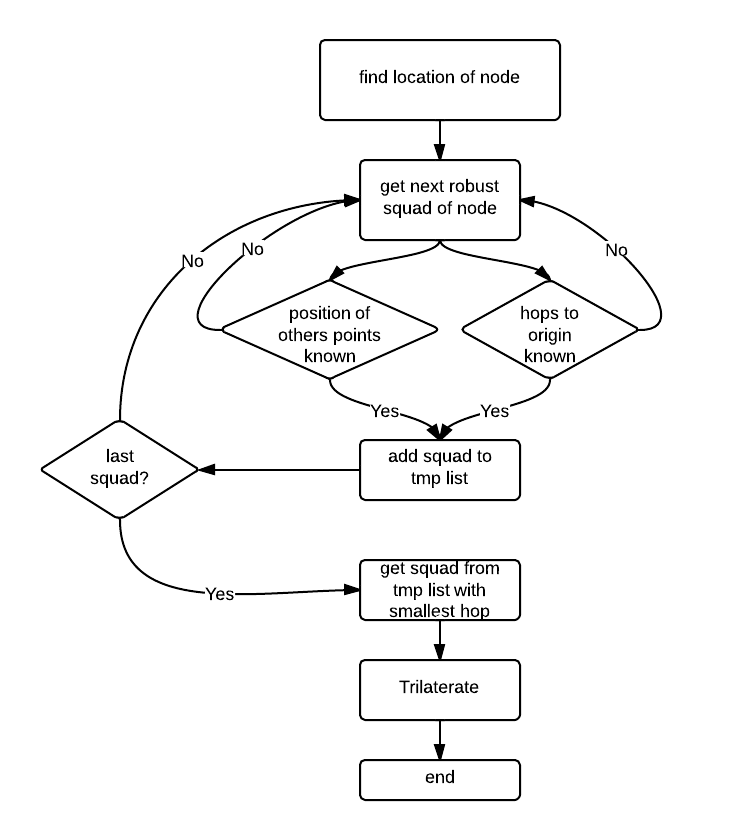
\includegraphics[width=90mm]{find_location.png}
\caption{find location of node}
\label{overflow}
\end{figure}

\subsection{Network configuration}
We tested our implementation against different types of networks configuration. The first and main one on is random graph with a minimum connectivity.
We also evaluated our solution with regular networks with particular properties.




\begin{thebibliography}{99}

\bibitem{c1} G. O. Young, ÒSynthetic structure of industrial plastics (Book style with paper title and editor),Ó 	in Plastics, 2nd ed. vol. 3, J. Peters, Ed.  New York: McGraw-Hill, 1964, pp. 15Ð64.




\end{thebibliography}




\end{document}